\documentclass[11pt]{article}

\usepackage[T1]{fontenc}
\usepackage[utf8]{inputenc}
\usepackage[sc]{mathpazo}
\usepackage{courier}
\linespread{1.04}
\usepackage{microtype}
\usepackage{placeins}
\usepackage[margin=1in]{geometry}
\usepackage{setspace}
\usepackage{amsmath,amssymb}
\usepackage{graphicx}
\usepackage{booktabs}
\usepackage{array}
\usepackage{threeparttable}
\usepackage[labelfont=bf]{caption}
\usepackage[authoryear,round]{natbib}
\usepackage{enumitem}
\usepackage{xcolor}
\usepackage[colorlinks=true,linkcolor=blue!50!black,citecolor=blue!50!black,urlcolor=blue!50!black]{hyperref}

\graphicspath{{figures/}}

% IRR macros remain conditional until independent human labels are available; do not synthesize kappa.
\newcommand{\fillin}[1]{\textcolor{red}{[#1]}}
% Inter-rater reliability: placeholders, overwritten by irr_numbers.tex, which
% P1_replication_package/paper_outputs/code/compute_interrater_reliability.py
% writes from the completed double-coding sheet.
\newcommand{\IRRN}{\fillin{N}}
\newcommand{\IRRAgree}{\fillin{agreement}}
\newcommand{\IRRKappa}{\fillin{kappa}}
\newcommand{\IRRModelAgree}{\fillin{model agreement}}
\newcommand{\IRRModelFone}{\fillin{macro-F1}}
\newcommand{\IRRSpecR}{\fillin{restrictive}}
\newcommand{\IRRSpecN}{\fillin{neutral}}
\newcommand{\IRRSpecS}{\fillin{supportive}}
\newif\ifIRR\IRRfalse
\InputIfFileExists{irr_numbers.tex}{}{}
\setlength{\bibsep}{2pt}
\captionsetup[table]{skip=6pt}
\captionsetup[figure]{skip=6pt}
\renewcommand{\arraystretch}{1.12}

\title{\textbf{Communication as Governance:}\\[2pt]
\textbf{Measuring Communicative Stance in University Intellectual Property Policies}}
\author{Working Paper}
\date{October 2026}

\begin{document}

\maketitle
\thispagestyle{empty}

\begin{abstract}
\noindent University intellectual-property policies allocate rights and communicate authority. We develop the Policy Communication Stance Index (PCSI), a human-anchored measure of supportive versus restrictive language based on 87,159 sentences from 518 source-document records at 150 U.S.\ research universities (1944--2025). Written stance leans restrictive: 86 percent of university-years fall below the scale midpoint. Stance varies persistently across universities, although observable characteristics explain relatively little. The index reflects supportive and obligation-oriented wording without reducing to readability, legal density, or measured rule form. Since 1980, stance has shifted toward restriction within universities, policy topics, and rule forms.

\vspace{0.8em}
\noindent\textbf{Keywords:} institutional governance; policy communication; university technology transfer; intellectual property; text as data; organizational heterogeneity

\noindent\textbf{JEL Codes:} O34, O38, I23, C55, K11
\end{abstract}

\newpage
\onehalfspacing

% =====================================================================
\section{Introduction}\label{sec:intro}

Universities govern faculty inventions through written policy. Intellectual-property policies specify who owns inventions, when they must be disclosed, how rights are assigned, and how licensing revenue is shared. Research on university patenting, licensing, and technology-transfer offices has examined these arrangements from several angles \citep{mowery2001growth,sampat2006patenting,jensen2003disclosure,ouellette2020patent}. A related literature studies academics' wider engagement with industry, which extends beyond licensing \citep{perkmann2021academic}. Even a prominent policy provision, the inventor's royalty share, has proven difficult to link reliably to commercialization: the positive association between royalty shares and licensing income reported by \citet{lach2008incentives} was subsequently challenged by \citet{ouellette2020patent}, who identified errors in the earlier coding and found no compelling evidence of a robust effect. Coding the terms of a policy may capture only part of what the policy conveys. The same disclosure or assignment rule can be written as a command or as an offer of assistance. This paper measures that second dimension in the written policies. It does not estimate its effects on inventor behavior or technology-transfer outcomes.

We call it \emph{communicative stance}. Organizational communication research treats formal texts as constitutive of organizations: they can speak for an institution and shape how readers understand its authority \citep{smith2001texts,cooren2004textual,fairhurst2004organizations,putnam2004alternative}. One policy may present disclosure as categorical compliance under unilateral authority; another may present a comparable requirement as part of a guided process with institutional assistance. Section~\ref{sec:framework} separates this relational framing from the regulative content of rules and develops the distinction into testable propositions. The distinction raises an economic question: can the wording of a fixed rule alter how costly or cooperative a reader expects the institutional process to be? Models and experiments on controlling incentives motivate that possibility, but do not test it for university IP policies \citep{benabou2003intrinsic,falk2006hidden}. Expressive accounts of law similarly draw attention to messages beyond formal sanctions \citep{sunstein1996expressive}. We use these literatures to motivate a simple mechanism, not to claim an observed behavioral effect. A useful related measurement approach, the survey-based Policy Communication Index of \citet{canary2013policy}, concerns communication practices and channels. Our object is narrower: the stance encoded in the formal policy text itself.

We construct the Policy Communication Stance Index (PCSI) from intellectual-property policies at 150 U.S.\ research universities over 1944--2025. The corpus contains 518 source-document records and 87,159 cleaned sentences, which yield 480 university-years with policy text and 4,277 annual policy-in-force observations. Human-coded sentences define restrictive, neutral, and supportive communication; a fine-tuned contextual classifier\footnote{A contextual classifier uses the words around a phrase when deciding its meaning. Fine-tuning means adapting a previously trained language model to the sentences labeled for this study.} scales those judgments to the full corpus; and calibrated class probabilities are aggregated to the university-year level. The approach follows the text-as-data literature's emphasis on defining the construct before scaling it statistically \citep{grimmer2013text,gentzkow2019text,adcock2001measurement}.

The analysis asks three questions. First, how do universities speak? Mean PCSI is 0.437, and 86.0 percent of policy-in-force observations lie below the neutral midpoint of 0.50: restrictive probability mass exceeds supportive mass in most policies. Validation exercises show that the measure tracks the supportive-versus-obligation dimension of policy wording rather than readability or legal-technical density, and that it is not reducible to the deontic form of rules as measured by keyword indicators: measured rule form explains under 5 percent of sentence-level variation in stance, and a version of PCSI net of it correlates 0.94 with the baseline.

Second, is stance changing? Average PCSI declines over the modern period, within fixed university cohorts and in years with source policy text. The decline is not confined to ownership and assignment clauses: negative trends also appear within disclosure, revenue-sharing, and administrative language, as well as within rule forms. An exact shift-share calculation for universities observed in both comparison periods attributes most of the decline to within-category changes, conditional on the chosen keyword classification. These descriptive comparisons do not establish effects of drafting changes on inventor behavior.

Third, who speaks differently? Stance is a persistent institutional attribute: 61.0 percent of variation in the annual panel, and 48.7 percent among years with source text, lies between universities. Private R1 universities write more supportive policies than public R1 universities, a difference of about 0.04 when policies written in the same year are compared, conditional on other characteristics. Land-grant status and other observable characteristics add little, and together they explain only a small share of cross-university differences.

The central contribution is to make a previously overlooked feature of university technology-transfer governance measurable: the way its formal rules address inventors. We define stance from human judgments, extend that definition to a large policy archive using a calibrated classifier, and check whether the resulting measure can be explained away by simple features of legal prose. The evidence shows that it cannot: universities differ in how they speak even within comparable rule forms, and the distribution of that language changes across decades. Section~\ref{sec:framework} sets out the conceptual framework, and Section~\ref{sec:measure} explains how PCSI is constructed and what it captures. Section~\ref{sec:results} reports its level, its evolution over time, and its institutional structure. Section~\ref{sec:discussion} discusses interpretation and limitations, and Section~\ref{sec:conclusion} concludes.

% =====================================================================
\section{Conceptual Framework: Policy Text as Governance}\label{sec:framework}

The communicative-constitution view of organizations holds that organizations exist in and through communication, and that written texts are able to circulate beyond the setting in which they were written. They can represent an institution long after their authors have moved on \citep{cooren2004textual,smith2001texts,putnam2004alternative,fairhurst2004organizations}. A university's intellectual-property policy is a text of this kind. It sets out expectations for inventors and may remain in use for many years, and it provides a formal statement of how invention rights will be handled. What a policy text does therefore has two parts: the rules it states, and the relationship between institution and reader that its wording enacts.

Institutional rules state what people are required or allowed to do. Yet the same rule can also suggest how an institution expects to relate to the people it governs \citep{crawford1995grammar,phillips2004discourse}. The Institutional Grammar describes institutional statements through five elements: who is addressed, the obligation or permission, the action, the conditions, and any consequence for noncompliance \citep{crawford1995grammar}. We study the language used to express those expectations. It is the part of a policy that tells inventors whether they are addressed as subjects of institutional control or as partners whom the institution will assist, and it can vary while the regulative content stays fixed. The distinction motivates three propositions about the texts, distinct from any claim about how inventors respond to them.

\begin{enumerate}[label=\textbf{P\arabic*.},leftmargin=2.2em,itemsep=2pt]
\item \textbf{Separability.} If framing is distinct from regulative content, stance should vary substantially among sentences with the same rule form, and a stance measure should not reduce to counts of obligations, prohibitions, and sanctions.
\item \textbf{Institutional persistence.} Texts become institutionalized when they are produced by actors with legitimate authority and are drawn on repeatedly by others \citep{phillips2004discourse}; studies of contracts suggest that formal language can be copied and changed incrementally, leaving traces of earlier drafts \citep{kahan1997standardization,choi2013dynamics}. Stance should therefore be a persistent, organization-specific attribute that broad organizational categories predict only weakly.
\item \textbf{Field-level drift.} Organizations in the same field can respond to shared legal and professional pressures and adopt similar forms \citep{dimaggio1983iron,edelman1992legal}. If such pressures change the register in which universities write, we would expect changes across multiple universities and parts of their policies, not only in the clauses that a particular legal event touches.
\end{enumerate}

A simple reader-engagement model (Appendix~\ref{app:comms-model}) makes the possible economic channel explicit: two equally demanding legal rules might communicate different expected procedural burdens. It is an illustration, not a fitted behavioral explanation of PCSI.

Table~\ref{tab:framework} summarizes where each proposition is examined. P1 is a condition for the measure to be meaningful and is tested in Section~\ref{sec:captures}; P2 and P3 are tested in Sections~\ref{sec:institutions} and~\ref{sec:time}. What follows tests features of the texts, not the engagement model or the effects of communication on technology-transfer outcomes.

\begin{table}[htbp]
\centering
\small
\caption{Framework Propositions and Where They Are Examined}
\label{tab:framework}
\begin{threeparttable}
\begin{tabular}{>{\raggedright\arraybackslash}p{0.18\textwidth}>{\raggedright\arraybackslash}p{0.36\textwidth}>{\raggedright\arraybackslash}p{0.36\textwidth}}
\toprule
Proposition & Observable implication & Evidence in this paper \\
\midrule
P1. Separability & Stance varies within rule forms; PCSI is not a count of obligations & Keyword-measured rule form explains 4.8\% of sentence-level stance; PCSI net of rule form correlates 0.94 with PCSI (Section~\ref{sec:captures}) \\
P2. Persistence & Stance is university-specific, revised incrementally, weakly predicted by categories & About half of variation is between universities; median revision 0.021; observables explain at most a sixth (Section~\ref{sec:institutions}) \\
P3. Field-level drift & Decline within universities, clause topics, and rule forms & Within-university decline; most balanced-sample change occurs within categories (Section~\ref{sec:time}) \\
\bottomrule
\end{tabular}
\end{threeparttable}
\end{table}

\FloatBarrier

% =====================================================================
\section{Measuring the Policy Communication Stance Index}\label{sec:measure}

The measurement task is to convert a qualitative feature of governance---how a university communicates authority, obligation, and support---into a comparable university-year score. We define the policy text and the unit being measured, anchor communicative stance in human sentence judgments, use a contextual classifier to extend those judgments to the full corpus, and aggregate the resulting probabilities into PCSI. We then ask what the index captures.

\subsection{Policy Texts and the Unit We Measure}

The corpus covers university intellectual-property policies from 150 U.S.\ research universities between 1944 and 2025: 87,159 cleaned sentences from 518 institution--year--file source-document records. These documents govern central parts of the university--inventor relationship, including ownership, disclosure, assignment, licensing authority, commercialization procedures, and revenue distribution.

A university can have more than one relevant policy document in the same year. In those cases we combine the sentences from documents covering the same university and year before computing its score, which yields 480 university-years with source policy text. Between observed source years, we carry forward the most recent observed policy score until a newer policy document appears\footnote{Carrying forward a score assumes that the observed policy remains in effect until another version is available. It does not mean a fresh document was found every year.}. Applying this rule through 2025 produces 4,277 annual policy-in-force university-years. These rows are annual representations of policies in force, not independently collected documents; each retains the source year from which its score is derived, so analyses can always separate the annual panel from the 480 source-text years. Table~\ref{tab:sample} summarizes the sample, and Appendix~\ref{app:data} documents the panel construction.

\begin{table}[htbp]
\centering
\small
\caption{Corpus and Analysis Sample, 1944--2025}
\label{tab:sample}
\begin{threeparttable}
\begin{tabular}{lr}
\toprule
Quantity & Value \\
\midrule
Universities & 150 \\
Analysis period & 1944--2025 \\
Source policy documents & 518 \\
Cleaned sentences & 87,159 \\
University-years with source policy text & 480 \\
Annual policy-in-force university-years & 4,277 \\
\bottomrule
\end{tabular}
\begin{tablenotes}[flushleft]\footnotesize
\item \textit{Notes:} When several source documents are available for the same university and year, their sentences are pooled before the university-year score is constructed. In the annual panel, that score is carried forward until a newer policy source becomes available.
\end{tablenotes}
\end{threeparttable}
\end{table}


\subsection{Defining Communicative Stance with Human Judgments}

We define communicative stance as the supportive, neutral, or restrictive presentation of institutional rights, obligations, authority, and assistance in formal policy text. The construct concerns how governance is expressed. It is not the substantive generosity of the underlying legal rule, generic positive or negative sentiment, or a measured response of faculty readers.

Human annotation turns this distinction into a labeling rule.\footnote{Annotation means assigning labels to examples by hand. Adjudication means reviewing disagreements and settling on a final label.} Supportive sentences emphasize assistance, guidance, encouragement, collaboration, shared interests, or facilitation. Restrictive sentences emphasize mandatory assignment, categorical obligations, unilateral authority, prohibitions, sanctions, or compliance. Neutral sentences are primarily definitional, descriptive, or procedural without a clear supportive or restrictive orientation. Coders classify the dominant message of the complete sentence, and disagreements were resolved through human adjudication. \ifIRR To assess reliability, two trained coders independently labeled a fresh random sample of \IRRN{} corpus sentences, blind to the classifier's predictions. They agreed on \IRRAgree{} percent of sentences (Cohen's $\kappa$ of \IRRKappa), and after adjudication the classifier's most likely label matched the human label for \IRRModelAgree{} percent (Appendix~\ref{app:model}).\else{} The coder-level records from the original annotation are not preserved, so historical inter-rater reliability statistics are not reported; the replication package includes a random double-coding sample and protocol so that reliability can be assessed independently (Appendix~\ref{app:model}).\fi

Rule content and communicative stance need not coincide. A disclosure requirement can be framed as categorical compliance or as part of a guided process, and a technically dense sentence can be supportive while a simple one communicates strong institutional control. Table~\ref{tab:examples} gives examples from the scored corpus; the last two rows are disclosure provisions written with opposite stance. Appendix~\ref{app:model} provides the annotation rubric and the reproducibility boundary of the preserved labels.

\begin{table}[htbp]
\centering
\small
\caption{Illustrative Sentence-Level Communicative Stance}
\label{tab:examples}
\begin{threeparttable}
\begin{tabular}{p{0.13\textwidth}p{0.67\textwidth}c}
\toprule
Class & Illustrative sentence & $\hat p_{\text{class}}$ \\
\midrule
Supportive & ``Inventors are encouraged to consult with the OTT concerning their options regarding the release of intellectual property.'' [Public R1, land-grant, 2012] & 0.973 \\
Neutral & ``Special procedures relevant to these processes are posted on the website of the Office of the Vice President for Research and Innovation.'' [Public R1, 2021] & 0.980 \\
Restrictive & ``As a condition of affiliation with the University, members of the University community are bound by all University policies, including this one.'' [Private R1, 2005] & 0.982 \\
\midrule
\multicolumn{3}{l}{\textit{Same disclosure obligation, different framing}} \\
Supportive & ``The University intends that the obligation for disclosure shall not unduly interfere with prompt publication of research results.'' [Public R1, 2010] & 0.975 \\
Restrictive & ``\ldots\ Each Invention must be disclosed promptly upon its creation, conception or discovery.'' [Public R1, 2013] & 0.978 \\
\bottomrule
\end{tabular}
\begin{tablenotes}[flushleft]\footnotesize
\item \textit{Notes:} $\hat p_{\text{class}}$ is the calibrated model probability assigned to the displayed class. Brackets give the institutional type and source year; institutions are identified in the replication package. The last two rows both state a disclosure obligation. The examples illustrate the annotation construct; they are not an independent accuracy test.
\end{tablenotes}
\end{threeparttable}
\end{table}


\subsection{Scaling the Human Judgments to the Full Corpus}

Human coding defines the classification target but cannot feasibly be applied manually to more than 87,000 sentences. We therefore use supervised natural-language processing as a scaling device. The preserved classifier is a fine-tuned \texttt{bert-base-uncased} model \citep{devlin2019bert}. A contextual model helps because the meaning of words such as \emph{shall}, \emph{may}, \emph{support}, or \emph{assign} depends on surrounding language.

The preserved labeled sample contains 2,732 sentences: 2,458 for training and 274 held out for validation. The model metadata reports 90.1 percent accuracy and 0.894 macro-F1 on a held-out validation set; these historical training-run metrics have not been independently re-estimated because the original labeled records were not retained.\footnote{Accuracy is the fraction of held-out sentences whose predicted class matches its human label. Precision is the share of a class's predictions that are correct, and recall is the share of that class's actual sentences recovered. The F1 statistic is their harmonic mean. Macro-F1 averages the three class-specific F1 scores equally, so a common class cannot dominate the statistic.} The model returns a probability distribution over restrictive, neutral, and supportive stance for every sentence, and we apply post-hoc temperature scaling\footnote{Temperature scaling adjusts a model's reported probabilities using a single fitted parameter. It does not change which class has the highest score.} before aggregation \citep{guo2017calibration}. Appendix~\ref{app:model} reports the configuration and calibration parameter.

\subsection{From Sentence Probabilities to PCSI}

Let $(\hat p_{Ri}, \hat p_{Ni}, \hat p_{Si})$ denote the calibrated restrictive, neutral, and supportive probabilities for sentence $i$. Placing restrictive communication at 0, neutral at 0.5, and supportive at 1, the continuous sentence score is
\begin{equation}
s_i = 0.5\,\hat p_{Ni} + \hat p_{Si}.
\end{equation}
A sentence with probability concentrated on the supportive class receives a value near 1, one concentrated on the restrictive class a value near 0, and one concentrated on the neutral class a value near 0.5. For university $j$ in year $t$, baseline PCSI is the unweighted mean of sentence scores in the pooled policy text,
\begin{equation}
\text{PCSI}_{jt} = \frac{1}{N_{jt}}\sum_{i=1}^{N_{jt}} s_i = 0.5 + 0.5\left(\bar{\hat p}_{S} - \bar{\hat p}_{R}\right)_{jt}.
\end{equation}
The range is $[0,1]$. Values below 0.5 indicate that restrictive probability mass exceeds supportive mass on average across the policy. A value of 0.5 does not require every sentence to be neutral; it can also result from offsetting supportive and restrictive mass.

\subsection{What the Measure Captures}\label{sec:captures}

Before interpreting PCSI substantively, we ask whether it depends on how sentence scores are combined, which recognizable features of policy language it reflects, and whether it merely restates the form of the rules a policy contains.

\paragraph{Aggregation.} We reconstruct the policy score using the within-policy median, a 5-percent trimmed mean, and a sentence-length-weighted mean. The trimmed and length-weighted versions remain very close to the baseline ($r = 0.999$ and $0.930$), while the median preserves much of the ranking (Spearman $\rho = 0.878$) but changes cardinal distances more noticeably (Appendix~\ref{app:robust}).

\paragraph{Linguistic content.} We construct three transparent diagnostics from the same text. \emph{Tone} summarizes supportive and collaborative language relative to obligation-, control-, and sanction-oriented wording. \emph{Clarity} summarizes sentence structure and procedural guidance. \emph{Legal Load} summarizes legal and IP-technical terminology (Appendix~\ref{app:linguistic}). The diagnostics are not alternative definitions of stance and do not enter PCSI. If PCSI captures the construct defined above, it should be related most strongly to Tone and should not reproduce readability or legal density.

Table~\ref{tab:linguistic} confirms this pattern. Entered alone, Tone accounts for 21.6 percent of in-sample variation in PCSI. Adding Clarity leaves the fit unchanged, and adding Legal Load raises $R^2$ to 0.236. Because nested $R^2$ comparisons depend on the order of entry, the table also reports Shapley shares\footnote{A Shapley share allocates the model's in-sample explained variation across predictors. With three diagnostics, it considers all six possible entry orders and averages each diagnostic's incremental increase in $R^2$. This is a description of explanatory fit, not a causal contribution.}, which average each diagnostic's marginal contribution over all orderings \citep{groemping2006relative}: Tone accounts for 89 percent of the explained variation, Legal Load for 9 percent, and Clarity for 2 percent. Using only the 480 source-text university-years, Tone's share is 78 percent. Tone and Legal Load are nearly uncorrelated ($r = 0.029$), so a policy can be technically dense while communicating assistance, and a simple policy can communicate categorical control. The three diagnostics together explain about a quarter of PCSI; the remainder may reflect combinations of language that lexical measures miss, such as discretion, relational framing, or the sequencing of obligations and assistance, as well as measurement error.

\begin{table}[htbp]
\centering
\small
\caption{Interpreting PCSI with Transparent Linguistic Features}
\label{tab:linguistic}
\begin{threeparttable}
\begin{tabular}{lccc}
\toprule
 & (1) & (2) & (3) \\
\midrule
Tone Index & 0.064*** & 0.063*** & 0.062*** \\
 & (0.012) & (0.012) & (0.012) \\
Clarity Index &  & 0.001 & 0.006 \\
 &  & (0.008) & (0.008) \\
Legal Load Index &  &  & 0.013** \\
 &  &  & (0.006) \\
\midrule
$R^2$ & 0.216 & 0.216 & 0.236 \\
Shapley share of $R^2$: Tone / Clarity / Legal Load & & & 0.89 / 0.02 / 0.09 \\
\quad Same, years with source text & & & 0.78 / 0.14 / 0.09 \\
Observations & 4,277 & 4,277 & 4,277 \\
\bottomrule
\end{tabular}
\begin{tablenotes}[flushleft]\footnotesize
\item \textit{Notes:} Dependent variable is policy-in-force PCSI; 150 universities. Standard errors clustered by university are in parentheses. Shapley shares average each index's marginal contribution to $R^2$ over all orders of entry and sum to one. Each diagnostic combines standardized components, so one unit of a composite should not be read as one standard deviation of that composite. *** $p<0.01$; ** $p<0.05$; * $p<0.10$.
\end{tablenotes}
\end{threeparttable}
\end{table}


\paragraph{Rule form versus framing.} A stronger concern is that PCSI simply counts rules: a policy full of obligations might score as restrictive regardless of how it states them. Inspired by the Institutional Grammar of \citet{crawford1995grammar}, we use keyword rules to classify each sentence by a deontic operator\footnote{A deontic operator is wording that expresses an obligation, permission, or prohibition. Our keyword rules do not code all five elements of the Institutional Grammar.}---obligation (\emph{shall}, \emph{must}, \emph{is required}), prohibition (\emph{shall not}, \emph{may not}), permission (\emph{may}, \emph{is entitled}), or none---and flag sanction language, the grammar's ``or else'' component. Obligations are the most restrictive form on average (mean sentence score 0.329, against 0.467 for sentences without a deontic operator), but the variation within forms dwarfs the differences between them: the eight form-by-sanction cells explain only 4.8 percent of sentence-level variance in stance (Appendix Table~\ref{tab:rule-form}). Prohibitions are no more restrictive than permissions on average, a reminder that a sentence's deontic operator says little about how it is framed. Subtracting each sentence's cell mean before aggregation yields a measure of framing net of rule form that correlates 0.94 with baseline PCSI and reproduces every headline result below (Appendix~\ref{app:uncertainty}). PCSI is therefore not reducible to these measured rule-form indicators. The indicators record deontic operators and sanction language, not the full substantive content of the obligations a sentence imposes, so the exercise shows that stance is not a count of musts and mays; it does not establish that framing has been fully separated from legal content.

These exercises define the scope of the measure. PCSI is a property of formal policy text. It is not a measure of substantive legal generosity, faculty perceptions, actual technology-transfer practice, or commercialization performance.

% =====================================================================
\section{The Empirical Structure of Communicative Stance}\label{sec:results}

We now describe the measure's level, its evolution over time, and its distribution across universities. The analyses are descriptive; none treats institutional characteristics or policy language as causes.

\subsection{PCSI Lies Below the Neutral Midpoint}

Figure~\ref{fig:hist} plots PCSI across the 4,277 policy-in-force university-years, and Table~\ref{tab:dist} reports summary statistics. Mean PCSI is 0.437, the median is 0.427, and the standard deviation is 0.066. The interquartile range runs from 0.394 to 0.471, with observed values from 0.264 to 0.730.

The central distributional result is the location of the mass relative to the scale midpoint: 86.0 percent of annual observations lie below 0.50. Because PCSI equals $0.5 + 0.5(\bar{\hat p}_S - \bar{\hat p}_R)$, a value below 0.50 means that restrictive probability mass exceeds supportive mass on average across the policy. It does not mean that every sentence is restrictive or that the underlying rules are unfavorable to inventors. The scale also contains meaningful dispersion: a one-standard-deviation difference in PCSI corresponds to a 0.132 difference in the average supportive-minus-restrictive margin, and the right tail extends to 0.730, showing that substantially more facilitative communication is possible within the same policy genre.

The pattern does not arise from carrying scores forward. Among the 480 university-years with source policy text, mean PCSI is 0.429 and 89.6 percent fall below 0.50. The midpoint is a scale reference, not a normative benchmark.

\begin{table}[htbp]
\centering
\small
\caption{Distribution of PCSI}
\label{tab:dist}
\begin{threeparttable}
\begin{tabular}{lcc}
\toprule
 & Policy-in-force panel & Years with source text \\
\midrule
Mean & 0.437 & 0.429 \\
Median & 0.427 & 0.423 \\
Standard deviation & 0.066 & 0.063 \\
25th percentile & 0.394 & 0.391 \\
75th percentile & 0.471 & 0.464 \\
Minimum & 0.264 & 0.264 \\
Maximum & 0.730 & 0.730 \\
Share below 0.50 & 86.0\% & 89.6\% \\
\midrule
Observations & 4,277 & 480 \\
\bottomrule
\end{tabular}
\begin{tablenotes}[flushleft]\footnotesize
\item \textit{Notes:} The policy-in-force panel carries each university's most recent score forward until a newer policy source appears; the second column uses only university-years for which policy text is directly available. Analysis window 1944--2025; 150 universities.
\end{tablenotes}
\end{threeparttable}
\end{table}


\begin{figure}[htbp]
\centering
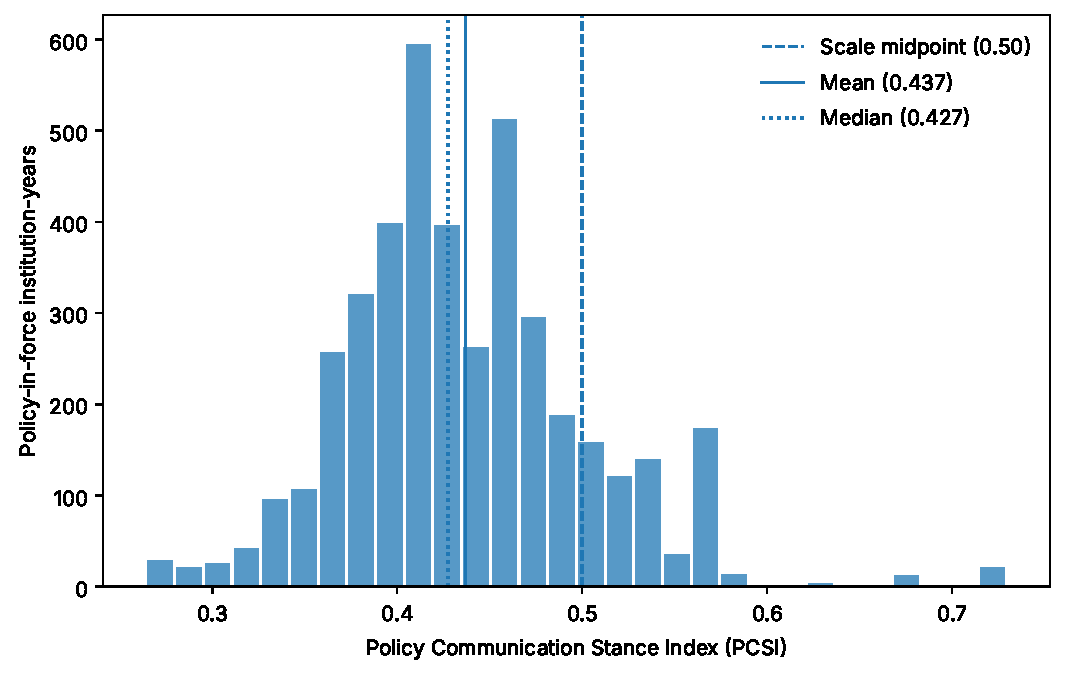
\includegraphics[width=0.82\textwidth]{fig1_pci_histogram.pdf}
\caption{Distribution of PCSI in the 1944--2025 Policy-in-Force Panel ($N = 4{,}277$). The dashed line marks the scale midpoint of 0.50; the solid and dotted lines mark the mean and median.}
\label{fig:hist}
\end{figure}

\subsection{PCSI Drifts Toward Restriction Over the Modern Period}\label{sec:time}

Figure~\ref{fig:trend} plots annual mean PCSI beginning in 1978, the first year in which at least five universities are represented. Average stance is highest around 1980, at roughly 0.49, and declines over subsequent decades to approximately 0.421 in 2025.

The raw series combines changes in policy language with changes in which universities the archive covers. Within fixed university cohorts the decline persists. Among the 93 universities already represented by 2000, mean PCSI falls from 0.447 to 0.422 by 2025, and the university fixed-effects\footnote{University fixed effects compare observations within each university after accounting for stable differences between universities.} trend is $-0.00112$ per year (clustered SE $= 0.00042$, $p = 0.008$). Cohorts beginning in 1990, 1995, and 2005 show the same pattern (Appendix Table~\ref{tab:cohorts}). Removing carry-forward and using only the 467 source-text university-years dated 1980 or later gives a fixed-effects trend of $-0.00117$ (SE $= 0.00039$, $p = 0.003$); starting in 1990 gives a similar estimate, while the post-2000 estimate is negative but less precise (Appendix Table~\ref{tab:observed-trends}).

\begin{figure}[htbp]
\centering
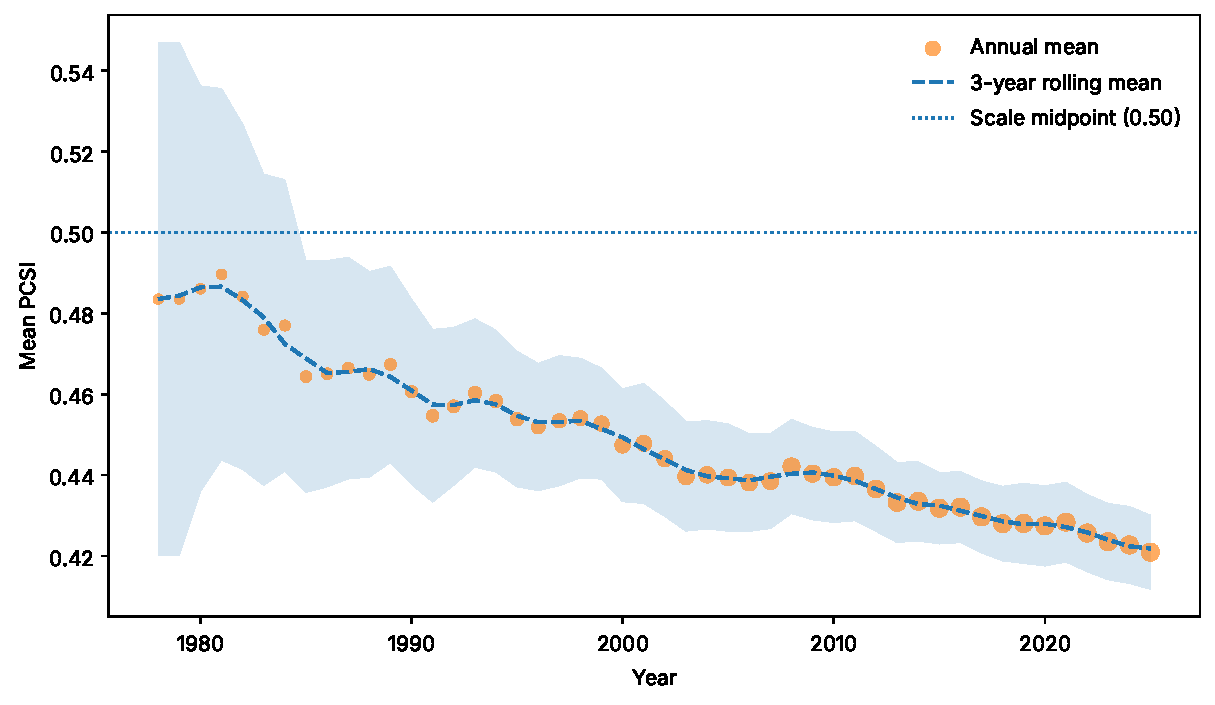
\includegraphics[width=0.86\textwidth]{fig3_temporal_trend_pcsi.pdf}
\caption{Annual Mean PCSI, 1978--2025. Points show annual cross-sectional means in the policy-in-force panel, with point size proportional to the number of universities represented. The shaded band is the 95\% confidence interval for the annual mean, the dashed line is the three-year rolling mean, and the dotted horizontal line marks the scale midpoint of 0.50. Years before 1978 are omitted because fewer than five universities are represented.}
\label{fig:trend}
\end{figure}

\paragraph{Is the decline a change in rules or in stance?} One explanation for the drift is substantive change in the underlying rules. The Supreme Court's decision in \emph{Stanford v.\ Roche} (2011) drew an important distinction between a promise to assign patent rights and a present assignment of those rights.\footnote{See \emph{Board of Trustees of the Leland Stanford Junior University v.\ Roche Molecular Systems, Inc.}, 563 U.S. 776 (2011), \url{https://www.law.cornell.edu/supremecourt/text/09-1159}. The decision establishes a distinction between assignment formulations; it does not, by itself, establish how many universities subsequently revised their policies.} Ownership and assignment clauses are also among the most restrictive in our corpus. If drafting changes were concentrated in such clauses, a fall in the index might mainly reflect their content. We therefore compare language within several policy topics and rule forms, without assuming the keywords fully recover legal meaning.

First, we assign sentences to clause topics with transparent keyword rules---ownership and assignment, disclosure, revenue sharing, licensing and commercialization, sponsored research, copyright and software, administration and disputes, and definitions (Appendix~\ref{app:topics})---and estimate university fixed-effects trends in mean sentence score within each topic, using source-text years from 1980. Figure~\ref{fig:topics} shows that the decline is broad. The trend in ownership and assignment language is close to zero ($-0.0003$ per year, $p = 0.64$), while disclosure ($-0.0022$, $p = 0.04$), revenue sharing ($-0.0017$, $p = 0.01$), and administrative language ($-0.0013$, $p = 0.02$) move toward restriction, and every other topic has a negative point estimate.

Second, we distinguish within-category changes in stance from changes in the composition of policy language. We use the 63 universities with source text in both 1980--1999 and 2010--2025. Each university contributes equally, regardless of its number of sentences. We compute the difference in its mean sentence score between periods, then partition that difference using symmetric within-category and composition components. The category contributions sum to the exact change for each university; we average those components only after performing the decomposition at the university level. The exercise uses one \emph{primary} topic per sentence, determined by fixed keyword priority, with unmatched sentences assigned to an ``other'' category; the separate topic-trend regressions above continue to allow overlapping matches. For rule form, each sentence belongs to one of the eight exclusive deontic-by-sanction cells. Appendix Table~\ref{tab:decomp} states how missing cells are handled and reports the numerical results.

The mean PCSI of these universities declined by 0.02882 (from 0.45545 to 0.42664). In the primary-topic decomposition, changes in the average stance \emph{within} categories contribute $-0.02223$, or 77.1\% of the observed decline; changes in category shares contribute $-0.00659$, or 22.9\%. In the separate eight-cell rule-form decomposition, within-cell changes contribute $-0.02708$ (94.0\%) and composition contributes $-0.00174$ (6.0\%). Both splits reproduce the observed change exactly, university by university and in aggregate.

These are two alternative descriptions of the same sample change, not effects attributable to different treatments. The allocation depends on keyword priority, the balanced-university sample, the handling of categories absent in one period, and the equal-university weighting. Most importantly, a change within a keyword-defined category may still reflect a substantive revision of the underlying rules. The decomposition therefore supports a limited descriptive statement: the observed decline is not accounted for entirely, or even mostly, by changing shares of the categories measured here.

The topic-specific evidence indicates that the modern decline is not confined to ownership and assignment clauses. It also appears within multiple rule forms. Because topics and rule forms are measured with keyword indicators, these results do not rule out substantive legal changes within categories, and the precise within-category share depends on how the categories are defined.

\begin{figure}[htbp]
\centering
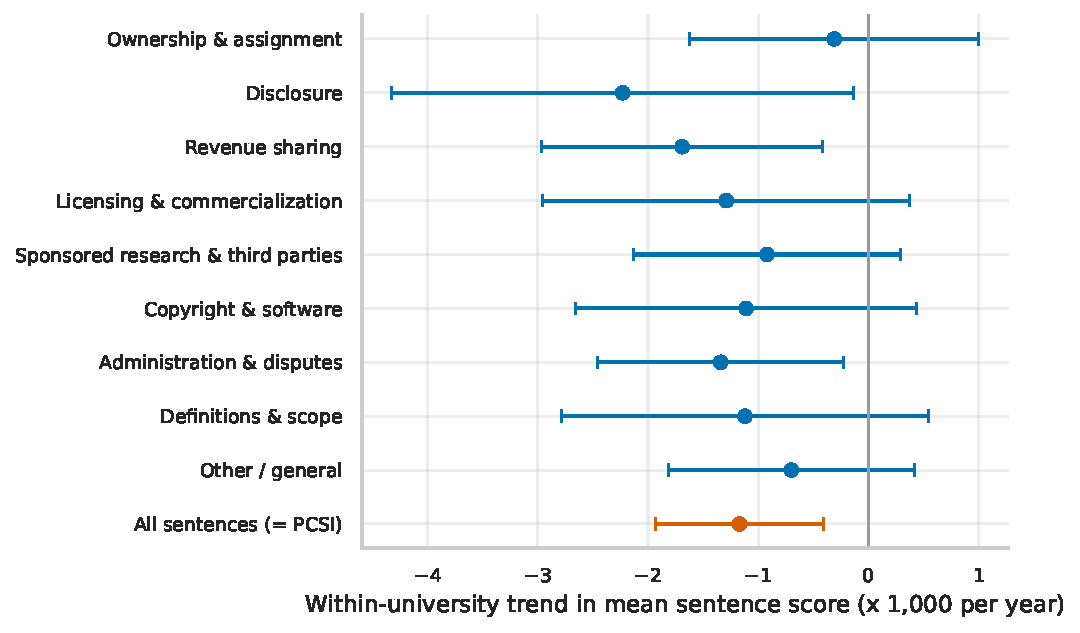
\includegraphics[width=0.82\textwidth]{fig_topic_trends.pdf}
\caption{Within-University Trends in Sentence Stance by Clause Topic, 1980--2025. Each point is the coefficient on year from a regression of the university-year mean sentence score within a topic on year and university fixed effects, using source-text university-years from 1980 onward and universities observed in at least two such years; coefficients are multiplied by 1,000. Bars are 95\% confidence intervals with university-clustered standard errors. Topics are assigned by keyword rules and can overlap (Appendix~\ref{app:topics}).}
\label{fig:topics}
\end{figure}

\subsection{Stance Is a Persistent Institutional Attribute, Weakly Explained by Observables}\label{sec:institutions}

\paragraph{Where the variation lies.} In the annual policy-in-force panel, 61.0 percent of the total sum of squared deviations in PCSI is between universities and 39.0 percent is within universities over time. Because the panel repeats a score until a newer source appears, carry-forward mechanically increases persistence; using only the 480 source-text university-years lowers the between-university share to 48.7 percent (Appendix Table~\ref{tab:variance}). Carry-forward matters for the magnitude, but it does not create the cross-university structure. Revisions are typically incremental: across 330 consecutive policy revisions within universities, the median absolute change in PCSI is 0.021. The pattern resembles a stable institutional writing style. This is an analogy to the persistent differences found in other organizational settings, not direct evidence about the people who drafted these policies \citep[compare][]{bertrand2003managing}.

\paragraph{Who speaks differently.} We next ask whether observable characteristics account for these differences.\footnote{R1 and R2 are research-activity categories in the Carnegie Classification of Institutions of Higher Education (methodology at \url{https://carnegieclassifications.acenet.edu/carnegie-classification/classification-methodology/}). The released metadata contains a binary \texttt{Carnegie R1} flag, and the analysis labels unflagged institutions R2; this R2 group is therefore an operational non-R1 category within the sample, not a certified match to an official R2 definition. The classification vintage behind the flag is not recorded. The 2021 Basic Classification assigns R1 and R2 using a multivariate research-activity index, whereas the 2025 research designations use explicit thresholds (at least \$50 million in R\&D expenditures and 70 research doctorates for R1; at least \$5 million and 20 research doctorates for R2), so the two vintages are not interchangeable. Institutional contrasts are therefore descriptive comparisons of the supplied groups, not reconstructions of official Carnegie categories. Control distinguishes public from private universities. Land-grant universities are those designated under the Morrill Acts of 1862 and 1890. Medical-school status indicates whether the university operates a medical school. Urbanicity groups campuses as rural, semi-urban, or city; without its original coding crosswalk it cannot be mapped to the locale framework of the National Center for Education Statistics. Region groups states into six U.S.\ regions. All classifications are time-invariant attributes recorded in the replication data.} Table~\ref{tab:inst-means} reports university-level means, where each university contributes the average of its annual scores so that institutions with longer archives do not receive more weight. We use rank-based tests because several groups are small (eight private R2 universities) and university means are skewed. Private R1 universities average 0.456, compared with 0.427 among public R1 universities (Kruskal--Wallis $p = 0.004$ across the four types). Land-grant universities average 0.420, compared with 0.442 among other institutions (Wilcoxon rank-sum $p = 0.010$). Both differences survive a Holm adjustment\footnote{The Holm procedure controls the probability of at least one false rejection within a specified family of tests by ordering their $p$-values and comparing them with successively less stringent thresholds. We apply it to the four stated institutional comparisons; it does not adjust for every exploratory specification in the paper.} across the four comparisons; medical-school status and urbanicity do not (Appendix Table~\ref{tab:holm}). Both directions hold under the alternative aggregations and when university means use only source-text years (Appendix~\ref{app:inst}).

\begin{table}[htbp]
\centering
\small
\caption{University-Level PCSI by Institutional Characteristics}
\label{tab:inst-means}
\begin{threeparttable}
\begin{tabular}{lcccc}
\toprule
Group & $N$ & Mean & SD & Range \\
\midrule
\multicolumn{5}{l}{\textit{Carnegie classification and control}} \\
\quad Private R1 & 38 & 0.456 & 0.046 & [0.337, 0.534] \\
\quad Public R1 & 86 & 0.427 & 0.051 & [0.328, 0.585] \\
\quad Private R2 & 8 & 0.406 & 0.053 & [0.342, 0.459] \\
\quad Public R2 & 18 & 0.441 & 0.058 & [0.376, 0.580] \\
\multicolumn{5}{l}{\textit{Mission and program}} \\
\quad Land-grant & 47 & 0.420 & 0.047 & [0.338, 0.585] \\
\quad Non-land-grant & 103 & 0.442 & 0.053 & [0.328, 0.580] \\
\quad Medical school & 118 & 0.438 & 0.053 & [0.328, 0.585] \\
\quad No medical school & 32 & 0.422 & 0.047 & [0.342, 0.519] \\
\multicolumn{5}{l}{\textit{Urbanicity}} \\
\quad Rural & 15 & 0.425 & 0.041 & [0.372, 0.519] \\
\quad Semi-urban & 48 & 0.422 & 0.047 & [0.338, 0.539] \\
\quad City & 82 & 0.443 & 0.057 & [0.328, 0.585] \\
\bottomrule
\end{tabular}
\begin{tablenotes}[flushleft]\footnotesize
\item \textit{Notes:} Unit of analysis is the university; PCSI is averaged across each university's policy-in-force years before group statistics are computed. Five universities lack urbanicity data. Rank-based tests are reported in Appendix~\ref{app:inst}.
\end{tablenotes}
\end{threeparttable}
\end{table}


Table~\ref{tab:inst-reg} considers the characteristics jointly. Columns (1)--(3) use university means. Relative to public R1 universities, the private-R1 coefficient is 0.029 (SE 0.009) with type alone, 0.019 with land-grant, medical-school, and urbanicity controls, and 0.020 (SE 0.014) with region fixed effects. The attenuation is not a sample artifact: Column (1) is unchanged at 0.029 when estimated on the 144 universities with complete covariates.

University means, however, mix institutional differences with the decades in which each university's policies were written, and with 144 observations they are imprecise. Column (4) instead uses the source-text university-years, includes source-year fixed effects so that each policy is compared with policies written in the same year, and clusters standard errors by university.\footnote{Clustering at the university level permits unexplained shocks to be correlated across observations of the same institution. It adjusts the estimated sampling uncertainty of the coefficients but not their point estimates; it does not remedy omitted variables or selection into the archive.} In this specification the private-R1 difference is 0.040 (SE 0.012) with all controls and region fixed effects, while the land-grant coefficient is $-0.005$ and imprecise. Weighting university means by the number of source policy years or sentences, or removing calendar-year means before averaging, leaves the qualitative pattern unchanged (Appendix Table~\ref{tab:inst-robust}).

\begin{table}[htbp]
\centering
\small
\caption{Institutional Correlates of PCSI}
\label{tab:inst-reg}
\begin{threeparttable}
\begin{tabular}{lcccc}
\toprule
 & \multicolumn{3}{c}{University means} & Source-text years \\
\cmidrule(lr){2-4}\cmidrule(lr){5-5}
 & (1) & (2) & (3) & (4) \\
\midrule
Private R1 & 0.029*** & 0.019 & 0.021 & 0.040*** \\
 & (0.009) & (0.012) & (0.014) & (0.012) \\
Private R2 & $-$0.021 & $-$0.031 & $-$0.035 & $-$0.006 \\
 & (0.021) & (0.023) & (0.023) & (0.018) \\
Public R2 & 0.014 & 0.007 & 0.011 & 0.005 \\
 & (0.015) & (0.020) & (0.018) & (0.011) \\
Land-grant &  & $-$0.014 & $-$0.011 & $-$0.005 \\
 &  & (0.012) & (0.013) & (0.012) \\
Medical school &  & 0.014 & 0.010 & 0.006 \\
 &  & (0.011) & (0.011) & (0.009) \\
\midrule
Urbanicity controls & No & Yes & Yes & Yes \\
Region fixed effects & No & No & Yes & Yes \\
Source-year fixed effects & No & No & No & Yes \\
$R^2$ & 0.074 & 0.111 & 0.161 & 0.291 \\
Observations & 150 & 145 & 144 & 452 \\
Universities & 150 & 145 & 144 & 144 \\
\bottomrule
\end{tabular}
\begin{tablenotes}[flushleft]\footnotesize
\item \textit{Notes:} Dependent variable is PCSI. Columns (1)--(3) use one observation per university (mean policy-in-force PCSI) with HC3 robust standard errors; Columns (2)--(3) omit universities with missing covariates. Column (4) uses university-years with directly available policy text, compares policies written in the same year through source-year fixed effects, and clusters standard errors by university. Public R1, rural, and Midwest are the omitted categories. *** $p<0.01$; ** $p<0.05$; * $p<0.10$.
\end{tablenotes}
\end{threeparttable}
\end{table}


Among these institutional comparisons, the private-R1 difference is the clearest regularity. The unconditional land-grant difference shrinks after adjusting for overlapping characteristics. Even so, observable characteristics explain at most about a sixth of cross-university variation in average PCSI. Broad institutional categories organize some communicative variation without determining it.

% =====================================================================
\section{Discussion}\label{sec:discussion}

The striking result is not simply that mandatory language is common. It is that the way universities communicate authority differs markedly across institutions and becomes more restrictive over time, even when we compare broadly similar categories of provisions. Our contribution is measurement and descriptive evidence; these differences are not evidence that language itself changes commercialization outcomes.

The communication-cost illustration gives one reason why two differently worded versions of the same requirement might be experienced differently by inventors. This corpus cannot tell us whether that happens. We observe policy wording, not readers' comprehension, disclosures, help-seeking, patents, or licensing outcomes; the model's behavioral parameter is unidentified. A paired drafting experiment or a policy revision linked to measured faculty responses would be needed to test it.

Persistence combined with weak observable correlates is what P2 predicts if stance reflects institution-specific drafting histories. Studies of corporate contracts and sovereign bonds find that legal language is often carried over and adapted from earlier documents \citep{kahan1997standardization,choi2013dynamics}. This offers one possible explanation for persistence in university policies, although those studies do not test university policy revisions. Shared legal and professional pressures could help explain the shift toward more restrictive wording \citep{dimaggio1983iron,edelman1992legal}; the evidence of drift within several keyword-defined clause topics and rule forms is consistent with a change in drafting register. The exact descriptive decompositions attribute most of the modern decline to within-category changes under the chosen definitions; they do not establish that the underlying legal content was unchanged or identify causal drivers. The institutional results fit the broader technology-transfer literature, which emphasizes heterogeneous professional routines, faculty--TTO relationships, and local commercialization practices \citep{owensmith2001patent,siegel2003assessing,bercovitz2008academic,perkmann2021academic}. PCSI adds a measurable textual dimension to that heterogeneity.

The annual panel assumes that the most recently available policy remains in force until a newer source is observed. Analyses restricted to years with source text reduce reliance on that assumption and yield the same central patterns, but they cannot establish that the historical archive is complete. The held-out validation set is small and does not establish accuracy separately by institution, period, or clause type. Sentence-level classification omits layout, headings, sequencing, and long-range relationships among passages, and the keyword rules used to assign topics and rule forms are transparent but coarse: they identify deontic operators and subject matter, not the full legal content of each provision. Downstream regressions use predicted rather than observed labels; the headline results are unchanged when PCSI is built from hard labels or from the two-thirds of sentences the model classifies with probability of at least 0.9, and model confidence is stable across decades (Appendix~\ref{app:uncertainty}). \ifIRR Because the double-coded reliability sample is linked to the scored corpus, it also makes formal corrections for generated variables \citep{egami2023using,battaglia2024inference} a natural extension.\else{} Independent double coding of the random reliability sample would help quantify label disagreement; additional inferential correction would depend on the assumptions and information required by the method selected \citep{egami2023using,battaglia2024inference}.\fi{} Most fundamentally, textual stance can diverge from substantive legal rights and from actual implementation. A higher PCSI should not be interpreted as a welfare ranking, a measure of legal generosity, or a recommendation to weaken legitimate disclosure and ownership requirements.

The replication package contains code for scoring, aggregating, building the annual panel, and producing every table, together with the canonical sentence scores and model metadata. The headline statistics, including the distribution, variance shares, fixed-effects trends, Shapley allocations, topic trends, institutional coefficients, and the within-versus-composition decompositions, have been recomputed from the canonical sentence-level data with code written independently of the original analysis scripts. These checks verify the released scores and the downstream calculations; they do not retrain the classifier. Because the original annotation and adjudication records were not preserved, the reported classifier performance metrics are those of the original training run rather than independently re-established validation statistics.\ifIRR{} A separately completed double-coding exercise provides reliability evidence distinct from the original training labels.\else{} Independent double coding of the distributed reliability sample remains to be completed.\fi

% =====================================================================
\section{Conclusion}\label{sec:conclusion}

This paper makes the communicative stance of university intellectual-property policy measurable. PCSI anchors supportive and restrictive language in human judgment, scales it with a calibrated classifier, and yields a panel covering 150 research universities over eight decades. The result is a contrast between stable institutional differences and gradual field-wide change. Most policies lean toward restrictive language. That pattern is not explained simply by the mix of obligations and permissions in the text; similar forms of rules can still be written in different registers. Since the 1980s, the register has become less supportive within universities and within several kinds of clauses. The measure describes policy wording, not the generosity of legal rights or the effectiveness of technology-transfer offices. It provides a consistent way to compare how universities communicate their rules, without treating differences in wording as evidence of differences in outcomes.

\section*{Data and Code Availability}

The released scored-sentence dataset, derived indices, analysis code, and saved tables are available in the \href{https://github.com/krish533/Tech-transfer-1/tree/main/P1_replication_package}{GitHub replication repository}.

\singlespacing
\bibliographystyle{plainnat}
\bibliography{references}

% =====================================================================
\newpage
\appendix
\onehalfspacing
\renewcommand{\thetable}{\thesection\arabic{table}}
\renewcommand{\thefigure}{\thesection\arabic{figure}}

\section{Data Construction and Sample Provenance}\label{app:data}
\setcounter{table}{0}

The analysis uses policy documents from 150 U.S.\ research universities over 1944--2025: 87,159 cleaned sentences from 518 institution--year--file source records. When more than one relevant document is available for the same university and year, the sentences are pooled before the university-year score is constructed, which yields 480 university-years with source policy text. The annual policy-in-force panel treats the most recently available score as remaining in force until a newer policy source appears for the same university; carrying scores forward through 2025 produces 4,277 annual observations. Each annual row retains the source year from which its score is derived. For cross-sectional comparisons, annual scores are averaged within university so that every university contributes one observation. The underlying archive also contains an isolated one-sentence 1925 record, retained for provenance but excluded from the analysis window.

\section{A Simple Model of Reader Engagement}\label{app:comms-model}

There is an economic reason to distinguish a rule from the way it is communicated, even when the university does not change the legal requirement. Consider an inventor deciding whether to initiate a conversation with the technology-transfer office. Let $r$ summarize the substantive rule, $s$ the stance that the inventor \emph{perceives} in its wording, and $c_i$ the inventor's opportunity cost of seeking guidance. Suppose the net value of engaging rather than remaining passive is
\begin{equation}\label{eq:communication-cost}
U_i(1)-U_i(0)=v(r)-c_i+\theta s+\varepsilon_i.
\end{equation}
The term $v(r)$ collects the legal and practical implications of the rule, while $\theta s$ represents a possible change in expected procedural burden or assistance associated with the wording. If $\varepsilon_i$ follows a logistic distribution with scale $\sigma>0$, the implied probability of engagement is
\begin{equation}\label{eq:engagement}
\Pr(a_i=1\mid r,s,c_i)=\Lambda\!\left(\frac{v(r)-c_i+\theta s}{\sigma}\right),\qquad
\Lambda(x)=\frac{1}{1+e^{-x}}.
\end{equation}
Holding the rule fixed, greater perceived support raises predicted engagement if $\theta>0$, has no effect if $\theta=0$, and could reduce it if the language feels untrustworthy ($\theta<0$).\footnote{The logistic expression is a simple choice-model illustration, not a fitted model. The sign of $\theta$ is not assumed or identified. $s$ denotes the reader's perceived stance; the text-based PCSI is only a possible empirical proxy for it, and no behavioral outcome is observed here.} None of these behavioral predictions is tested in the present data. The immediate empirical implication is more modest: \emph{the same measured rule form can have different communicative stance}. That is the separability question we can investigate with the policy corpus. A future reader experiment could hold the legal provision fixed, randomize supportive versus commanding wording, and measure comprehension, perceived burden, and willingness to request guidance. Such a design would test the mechanism without mistaking our descriptive index for a treatment effect.

\section{Annotation, Model, and Replication Provenance}\label{app:model}
\setcounter{table}{0}

\paragraph{Annotation rubric.} Sentences are classified as supportive, neutral, or restrictive. Supportive language emphasizes assistance, guidance, encouragement, collaboration, shared interests, or facilitation. Restrictive language emphasizes mandatory assignment, unilateral institutional authority, prohibitions, sanctions, forfeiture, or categorical compliance obligations. Neutral language is primarily definitional, descriptive, or procedural without a clear directional stance. The coding rule concerns the dominant communicative stance of the complete sentence. Multiple trained human coders applied the rubric, and disagreements were resolved through human adjudication. The preserved artifacts contain 2,732 adjudicated labeled sentences.

\ifIRR
\paragraph{Reliability.} The coder-level records from the original annotation are not preserved, so reliability is assessed on a fresh sample. We drew \IRRN{} sentences at random from the 1944--2025 corpus; two trained coders labeled each independently using the rubric above, without access to the classifier's predictions, and disagreements were adjudicated. Raw agreement between coders is \IRRAgree{} percent and Cohen's $\kappa$ is \IRRKappa. Specific agreement, the share of one coder's uses of a class matched by the other, is \IRRSpecR{} percent for restrictive, \IRRSpecN{} percent for neutral, and \IRRSpecS{} percent for supportive sentences. Against the adjudicated labels, the classifier's most likely label agrees for \IRRModelAgree{} percent of sentences, with macro-F1 of \IRRModelFone. The sampling and scoring code is \texttt{compute\_interrater\_reliability.py} in the replication package.
\else
\paragraph{Reliability.} The coder-level records from the original annotation are not preserved, so historical inter-rater reliability statistics cannot be reconstructed and are not reported. To allow reliability to be assessed independently of those records, the replication package includes a random sample of 400 corpus sentences, drawn without the classifier's predictions, together with coding instructions and the code that computes agreement, Cohen's $\kappa$, and classifier agreement once the sample has been double-coded (\texttt{compute\_interrater\_reliability.py}).
\fi

\paragraph{Classifier and calibration.} Table~\ref{tab:classifier} reports the configuration of the preserved classifier. Post-hoc temperature scaling is applied before probability aggregation. The replication package reproduces inference from the saved classifier, calibrated sentence scores, aggregation, panel construction, and the manuscript analyses; the original fine-tuning run cannot presently be reconstructed. Rescoring a random sample of 2,000 sentences with the preserved model and temperature reproduces the canonical calibrated probabilities to within $4\times10^{-6}$ and assigns the same label to every sentence. Every sentence score can also be reconstructed from the saved calibrated probabilities, and rebuilding the observed and policy-in-force university-year indices from those scores reproduces them to numerical precision.

\begin{table}[htbp]
\centering
\small
\caption{Preserved Classifier Configuration}
\label{tab:classifier}
\begin{threeparttable}
\begin{tabular}{lr}
\toprule
Parameter & Value \\
\midrule
Base model & \texttt{bert-base-uncased} \\
Transformer layers & 12 \\
Attention heads & 12 \\
Hidden size & 768 \\
Intermediate size & 3,072 \\
Maximum input length & 256 tokens \\
Output classes & 3 \\
Training sentences & 2,458 \\
Validation sentences & 274 \\
Total labeled sentences & 2,732 \\
Temperature parameter & $T = 0.8462$ \\
Validation accuracy & 0.901 \\
Validation macro-F1 & 0.894 \\
\bottomrule
\end{tabular}
\begin{tablenotes}[flushleft]\footnotesize
\item \textit{Notes:} Configuration and metrics are read from the preserved model artifacts in the replication package.
\end{tablenotes}
\end{threeparttable}
\end{table}


\section{Measurement Robustness}\label{app:robust}
\setcounter{table}{0}

Table~\ref{tab:aggregation} compares the baseline with the within-policy median, a 5-percent trimmed mean, and a sentence-length-weighted mean. Trimming changes almost nothing, length weighting remains strongly aligned with the baseline, and median aggregation produces the largest cardinal difference while retaining a Spearman correlation of 0.878. Table~\ref{tab:variance} repeats the between/within decomposition under each aggregation and in the 480 source-text years. Carry-forward increases measured persistence under every construction, but substantial cross-university structure remains without it.

\begin{table}[htbp]
\centering
\small
\caption{Sensitivity to Alternative Sentence Aggregation Rules}
\label{tab:aggregation}
\begin{threeparttable}
\begin{tabular}{lcccc}
\toprule
Aggregation & Mean & Pearson $r$ & Spearman $\rho$ & Midpoint agreement \\
\midrule
Baseline (unweighted mean) & 0.437 & 1.000 & 1.000 & 1.000 \\
Median PCSI & 0.471 & 0.623 & 0.878 & 0.937 \\
5\% trimmed mean & 0.431 & 0.999 & 1.000 & 1.000 \\
Length-weighted mean & 0.433 & 0.930 & 0.906 & 0.933 \\
\bottomrule
\end{tabular}
\begin{tablenotes}[flushleft]\footnotesize
\item \textit{Notes:} $N = 4{,}277$ policy-in-force university-years. Correlations are with baseline PCSI. Midpoint agreement is the share of observations that the baseline and the alternative place on the same side of 0.50.
\end{tablenotes}
\end{threeparttable}
\end{table}

\begin{table}[htbp]
\centering
\small
\caption{Between- and Within-University Variation}
\label{tab:variance}
\begin{threeparttable}
\begin{tabular}{lcc}
\toprule
Specification & Between share & Within share \\
\midrule
\multicolumn{3}{l}{\textit{Policy-in-force panel}} \\
\quad Baseline & 0.610 & 0.390 \\
\quad Median & 0.434 & 0.566 \\
\quad Trimmed mean & 0.616 & 0.384 \\
\quad Length-weighted mean & 0.589 & 0.411 \\
\multicolumn{3}{l}{\textit{Years with source text}} \\
\quad Baseline & 0.487 & 0.513 \\
\quad Median & 0.300 & 0.700 \\
\quad Trimmed mean & 0.494 & 0.506 \\
\quad Length-weighted mean & 0.463 & 0.537 \\
\bottomrule
\end{tabular}
\begin{tablenotes}[flushleft]\footnotesize
\item \textit{Notes:} Shares partition the total sum of squared deviations of PCSI into between- and within-university components.
\end{tablenotes}
\end{threeparttable}
\end{table}


\section{Institutional Tests}\label{app:inst}
\setcounter{table}{0}

Table~\ref{tab:holm} reports the four rank-based institutional comparisons with Holm-adjusted $p$-values. The unconditional patterns are stable across aggregation choices: the private-R1 minus public-R1 difference is 0.029 with baseline PCSI, 0.018 with the median, and 0.032 with both the trimmed and the length-weighted mean; the land-grant minus non-land-grant difference ranges from $-0.020$ to $-0.024$. When university averages use only source-text years, the two differences are 0.033 and $-0.019$.

\begin{table}[htbp]
\centering
\small
\caption{Institutional Comparisons with Multiple-Testing Adjustment}
\label{tab:holm}
\begin{threeparttable}
\begin{tabular}{llcc}
\toprule
Characteristic & Test & Raw $p$ & Holm $p$ \\
\midrule
Carnegie classification and control & Kruskal--Wallis & 0.004 & 0.014 \\
Land-grant status & Wilcoxon rank-sum & 0.010 & 0.029 \\
Urbanicity & Kruskal--Wallis & 0.055 & 0.111 \\
Medical-school status & Wilcoxon rank-sum & 0.172 & 0.172 \\
\bottomrule
\end{tabular}
\begin{tablenotes}[flushleft]\footnotesize
\item \textit{Notes:} University-level mean PCSI ($N=150$; 145 for urbanicity). The Holm adjustment is applied to this family of four tests.
\end{tablenotes}
\end{threeparttable}
\end{table}


Table~\ref{tab:inst-robust} reports the private-R1 and land-grant coefficients across samples, weights, and era adjustments. Archive vintage differs modestly by type: the mean source-policy year is 2002.3 for private R1 universities and 2005.1 for public R1 universities. Because PCSI declines over time, comparing university means without adjusting for era slightly favors universities with older archives, which is why Column (4) of Table~\ref{tab:inst-reg} compares policies within source year. The private-R1 difference is larger, not smaller, in that comparison.

\begin{table}[htbp]
\centering
\small
\caption{Private-R1 and Land-Grant Coefficients Across Samples and Estimators}
\label{tab:inst-robust}
\begin{threeparttable}
\begin{tabular}{lcccc}
\toprule
 & Type only & \multicolumn{2}{c}{Full controls} & \\
\cmidrule(lr){2-2}\cmidrule(lr){3-4}
 & Private R1 & Private R1 & Land-grant & $N$ \\
\midrule
University means & 0.029*** & 0.021 & $-$0.011 & 144 \\
 & (0.009) & (0.014) & (0.013) & \\
University means, common sample & 0.029*** & 0.021 & $-$0.011 & 144 \\
 & (0.009) & (0.014) & (0.013) & \\
WLS, weight = source policy years & 0.027** & 0.020 & $-$0.021 & 144 \\
 & (0.010) & (0.015) & (0.015) & \\
WLS, weight = sentences & 0.021 & 0.023 & 0.005 & 144 \\
 & (0.014) & (0.023) & (0.028) & \\
Era-adjusted university means & 0.029*** & 0.022 & $-$0.009 & 144 \\
 & (0.009) & (0.014) & (0.013) & \\
Source-text years, year FE & 0.040*** & 0.040*** & $-$0.005 & 452 \\
 & (0.010) & (0.012) & (0.012) & \\
Source-text years from 1980, year FE & 0.039*** & 0.038*** & $-$0.005 & 439 \\
 & (0.010) & (0.012) & (0.012) & \\
\bottomrule
\end{tabular}
\begin{tablenotes}[flushleft]\footnotesize
\item \textit{Notes:} Dependent variable is PCSI; public R1 is the omitted type. ``Full controls'' adds land-grant, medical-school, and urbanicity indicators and region fixed effects. University-mean rows use HC3 standard errors; the published row uses 150 universities for the type-only column and 144 with full controls. Era-adjusted means subtract each calendar year's cross-sectional mean from the policy-in-force panel before averaging within university. Source-text rows use university-years with directly available policy text, include source-year fixed effects, and cluster standard errors by university. *** $p<0.01$; ** $p<0.05$; * $p<0.10$.
\end{tablenotes}
\end{threeparttable}
\end{table}


\section{Transparent Linguistic Diagnostics}\label{app:linguistic}
\setcounter{table}{0}

The diagnostics interpret the supervised measure; they are not independent validation of reader perceptions or alternative definitions of stance. Let $z(\cdot)$ denote a standardized policy-level component. The indices are
\begin{align}
\text{Tone} &= \tfrac{1}{6}\big[z(\text{supportive}) + z(\text{second person}) + z(\text{inclusive we}) \notag\\
&\qquad - z(\text{restrictive}) - z(\text{sanction}) - z(\text{obligation modal share})\big],\\
\text{Clarity} &= \tfrac{1}{3}\big[-z(\text{mean sentence length}) - z(\text{long-sentence share}) + z(\text{procedural share})\big],\\
\text{Legal Load} &= \tfrac{1}{2}\big[z(\text{legalese}) + z(\text{IP technical})\big].
\end{align}
Supportive, restrictive, sanction, procedural, legalese, and IP-technical components are constructed from transparent dictionaries implemented in the replication code; second-person and inclusive-first-person components capture direct and collective interpersonal language. Components are normalized for policy length where appropriate and standardized before the composites are formed. The three diagnostics are empirically distinct: Tone and Clarity correlate at 0.143, Tone and Legal Load at 0.029, and Clarity and Legal Load at $-0.296$. Table~\ref{tab:length} shows that adding log word count or log sentence count leaves the Tone relationship almost unchanged while reducing the Legal Load coefficient. In the 480 source-text years, the three-index model gives coefficients of 0.038 for Tone, 0.013 for Clarity, and 0.012 for Legal Load, with $R^2 = 0.151$.

\begin{table}[htbp]
\centering
\small
\caption{Linguistic Decomposition with Policy-Length Controls}
\label{tab:length}
\begin{threeparttable}
\begin{tabular}{lccc}
\toprule
 & Baseline & + Log words & + Log sentences \\
\midrule
Tone Index & 0.062*** & 0.059*** & 0.059*** \\
 & (0.012) & (0.012) & (0.012) \\
Clarity Index & 0.006 & 0.006 & 0.008 \\
 & (0.008) & (0.008) & (0.009) \\
Legal Load Index & 0.013** & 0.010 & 0.010 \\
 & (0.006) & (0.007) & (0.007) \\
\midrule
Policy-length control & No & Log words & Log sentences \\
$R^2$ & 0.236 & 0.244 & 0.241 \\
Observations & 4,277 & 4,277 & 4,277 \\
\bottomrule
\end{tabular}
\begin{tablenotes}[flushleft]\footnotesize
\item \textit{Notes:} University-clustered standard errors in parentheses. *** $p<0.01$; ** $p<0.05$; * $p<0.10$.
\end{tablenotes}
\end{threeparttable}
\end{table}


\section{Temporal Robustness}\label{app:temporal}
\setcounter{table}{0}

The raw annual series can change because policy language changes or because the set of represented universities changes. Table~\ref{tab:cohorts} holds composition fixed using universities already represented by selected start years; every cohort has a lower mean in 2025 than at the start, and every university fixed-effects trend is negative. Table~\ref{tab:observed-trends} removes annual carry-forward and uses only university-years with source policy text. The 2025 cross-section is not driven by unusually old policies: among the 70 universities whose policy in force in 2025 is at most five years old, 91 percent lie below the midpoint, against 92 percent of all 150.

\begin{table}[htbp]
\centering
\small
\caption{PCSI Trends Within Fixed University Cohorts}
\label{tab:cohorts}
\begin{threeparttable}
\begin{tabular}{cccccc}
\toprule
Cohort start & Universities & Start mean & 2025 mean & FE trend per year & $p$ \\
\midrule
1990 & 34 & 0.461 & 0.421 & $-$0.00109 & 0.019 \\
1995 & 53 & 0.454 & 0.422 & $-$0.00131 & 0.002 \\
2000 & 93 & 0.447 & 0.422 & $-$0.00112 & 0.008 \\
2005 & 114 & 0.439 & 0.420 & $-$0.00103 & 0.011 \\
\bottomrule
\end{tabular}
\begin{tablenotes}[flushleft]\footnotesize
\item \textit{Notes:} Each cohort contains the universities already represented in the policy-in-force panel by the start year. Trends come from regressions of PCSI on year with university fixed effects; standard errors are clustered by university.
\end{tablenotes}
\end{threeparttable}
\end{table}

\begin{table}[htbp]
\centering
\small
\caption{Temporal Trends Using Only Years with Source Policy Text}
\label{tab:observed-trends}
\begin{threeparttable}
\begin{tabular}{cccccc}
\toprule
Start year & $N$ & Pooled trend & FE trend & SE & $p$ \\
\midrule
1980 & 467 & $-$0.00115 & $-$0.00117 & (0.00039) & 0.003 \\
1990 & 443 & $-$0.00121 & $-$0.00128 & (0.00053) & 0.016 \\
2000 & 367 & $-$0.00109 & $-$0.00150 & (0.00093) & 0.105 \\
\bottomrule
\end{tabular}
\begin{tablenotes}[flushleft]\footnotesize
\item \textit{Notes:} University-years with directly available policy text from the start year onward. Standard errors are clustered by university.
\end{tablenotes}
\end{threeparttable}
\end{table}


\section{Clause Topics and Rule Forms}\label{app:topics}
\setcounter{table}{0}

\paragraph{Clause topics.} Sentences are assigned to topics by case-insensitive keyword rules: ownership and assignment (\emph{assign}, \emph{ownership}, \emph{title}, \emph{vest}, \emph{belong}); disclosure (\emph{disclos}, \emph{invention report}); revenue sharing (\emph{royalt}, \emph{revenue}, \emph{net income/proceeds}, \emph{distribut}, \emph{equity}); licensing and commercialization (\emph{licens}, \emph{commerciali}, \emph{technology transfer}, \emph{start-up}, \emph{patent application}); sponsored research and third parties (\emph{sponsor}, \emph{grant}, \emph{federal}, \emph{government}, \emph{contract}, \emph{third part}); copyright and software (\emph{copyright}, \emph{software}, \emph{courseware}, \emph{scholarly work}); administration and disputes (\emph{appeal}, \emph{dispute}, \emph{committee}, \emph{review}, \emph{waive}, \emph{grievance}, \emph{amend}); and definitions and scope (\emph{means}, \emph{defined}, \emph{applies to}, \emph{purpose}, \emph{scope}). A sentence can belong to several topics, and the within-topic regressions retain those overlaps. For the decomposition alone, each sentence receives a single primary topic (the first matching category in the order listed); sentences with no match are classified as other/general. This distinction matters when comparing the two sets of findings. Among sentences from 1980 onward, 59 percent match at least one topic. Ownership and assignment sentences are the most restrictive (mean score 0.335), and definitional and revenue-sharing sentences the least (0.448 and 0.453). Table~\ref{tab:topics} reports within-topic trends.

\paragraph{Exact within-category and composition accounting.} The decomposition compares source-text sentences from 1980--1999 with those from 2010--2025 for the 63 universities that appear in both periods (8,353 early sentences and 28,175 late sentences). For university $i$, let $s_{ikt}$ be its fraction of sentences in mutually exclusive category $k$ and $m_{ikt}$ the category's mean stance score in period $t$, where $t\in\{0,1\}$. The university mean is $M_{it}=\sum_k s_{ikt}m_{ikt}$. Using the period-average category share and mean gives the exact identity
\begin{equation}\begin{split}
M_{i1}-M_{i0}
&= \underbrace{\sum_k \frac{s_{ik1}+s_{ik0}}{2}(m_{ik1}-m_{ik0})}_{\text{within-category change}}\\[2pt]
&\quad+\underbrace{\sum_k \frac{m_{ik1}+m_{ik0}}{2}(s_{ik1}-s_{ik0})}_{\text{composition change}}.
\end{split}\end{equation}
If a category is absent for a university in one period, its unobserved conditional mean is set equal to that category's mean in the period where it appears. This explicitly allocates category entry or exit to composition rather than within-category change. The choice is a convention, not an identified counterfactual. We perform the identity calculation within each university before averaging the contributions equally across universities; in particular, products of separately averaged university shares and means cannot replace averages of university-level products. Both independently recalculated decompositions reconcile to the observed mean change within numerical tolerance of $10^{-11}$. The topic decomposition uses one exclusive primary topic; the form decomposition uses eight exclusive deontic-by-sanction cells. These alternative breakdowns are not additive. Per-university contributions and the code that verifies the identity are included in the replication package.

\begin{table}[htbp]
\centering
\small
\caption{Exact Shift--Share Decompositions of the Modern PCSI Decline}
\label{tab:decomp}
\begin{threeparttable}
\begin{tabular}{lrr}
\toprule
 & Exclusive primary topic & Deontic $\times$ sanction \\
\midrule
Early period: mean score (1980--1999) & 0.455454 & 0.455454 \\
Late period: mean score (2010--2025) & 0.426638 & 0.426638 \\
\textbf{Observed change} & \textbf{$-0.028816$} & \textbf{$-0.028816$} \\
Within-category contribution & $-0.022229$ & $-0.027077$ \\
Composition contribution & $-0.006587$ & $-0.001739$ \\
Within-category share of decline & 77.1\% & 94.0\% \\
Composition share of decline & 22.9\% & 6.0\% \\
Universities with policies in both periods & 63 & 63 \\
Early and late sentences & 8,353; 28,175 & 8,353; 28,175 \\
\bottomrule
\end{tabular}
\begin{tablenotes}[flushleft]\footnotesize
\item \textit{Notes:} The unit of comparison is a university appearing in both periods; universities are weighted equally. Each sentence is assigned to one primary topic by fixed keyword priority, or to one of eight deontic-by-sanction cells. Category changes are decomposed within each university using midpoint shares and midpoint conditional means, then averaged. If a category is absent in a period, its conditional mean is imputed from the observed period, assigning category entry/exit to composition. The university-level accounting identity holds to machine precision. These alternative decompositions are not additive and are sensitive to the coding rules and missing-category convention. The numbers are descriptive, not causal estimates.
\end{tablenotes}
\end{threeparttable}
\end{table}


\paragraph{Rule forms.} Following \citet{crawford1995grammar}, each sentence receives one deontic operator, assigned with priority prohibition ($\neg$ \emph{shall}, \emph{must}, \emph{may}, \emph{will}, \emph{can}; \emph{cannot}; \emph{prohibit}; \emph{not permitted}) $>$ obligation (\emph{shall}, \emph{must}, \emph{is required}, \emph{requires}, \emph{obligat-}, \emph{agrees to}, \emph{is expected to}) $>$ permission (\emph{may}, \emph{permit}, \emph{entitled}, \emph{discretion}, \emph{can}, \emph{allow}) $>$ none. Sanction language (\emph{violat-}, \emph{disciplin-}, \emph{sanction}, \emph{forfeit}, \emph{terminat-}, \emph{breach}, \emph{penalt-}, \emph{dismiss}, \emph{revok-}) is flagged separately. Table~\ref{tab:rule-form} reports stance by form. At the policy level, the shares of obligation, prohibition, permission, and sanction sentences together explain 11 percent of the variation in PCSI across the 480 source-text university-years.

\begin{table}[htbp]
\centering
\small
\caption{Within-University Trends in Sentence Stance by Clause Topic, 1980--2025}
\label{tab:topics}
\begin{threeparttable}
\begin{tabular}{lccccc}
\toprule
Topic & Share & Mean score & FE trend per year & SE & $p$ \\
\midrule
Ownership \& assignment & 0.142 & 0.335 & $-$0.00031 & (0.00067) & 0.644 \\
Disclosure & 0.057 & 0.357 & $-$0.00223 & (0.00107) & 0.037 \\
Revenue sharing & 0.131 & 0.453 & $-$0.00169 & (0.00065) & 0.010 \\
Licensing \& commercialization & 0.133 & 0.432 & $-$0.00129 & (0.00085) & 0.129 \\
Sponsored research \& third parties & 0.131 & 0.341 & $-$0.00092 & (0.00062) & 0.140 \\
Copyright \& software & 0.092 & 0.412 & $-$0.00111 & (0.00079) & 0.159 \\
Administration \& disputes & 0.141 & 0.425 & $-$0.00134 & (0.00057) & 0.018 \\
Definitions \& scope & 0.083 & 0.448 & $-$0.00112 & (0.00085) & 0.185 \\
Other / general & 0.409 & 0.427 & $-$0.00070 & (0.00057) & 0.213 \\
\midrule
All sentences (= PCSI) & 1.000 &  & $-$0.00117 & (0.00039) & 0.002 \\
\bottomrule
\end{tabular}
\begin{tablenotes}[flushleft]\footnotesize
\item \textit{Notes:} Each row regresses the university-year mean sentence score within a topic on year and university fixed effects, using source-text university-years from 1980 and universities observed in at least two such years; standard errors are clustered by university. Topics are assigned by keyword rules and can overlap; share is the fraction of 1980--2025 sentences matching the topic. Shift-share for the 63 universities with source text in both 1980--1999 and 2010--2025: within-topic change $-$0.028, change in topic composition $-$0.003.
\end{tablenotes}
\end{threeparttable}
\end{table}

\begin{table}[htbp]
\centering
\small
\caption{Communicative Stance by Rule Form}
\label{tab:rule-form}
\begin{threeparttable}
\begin{tabular}{lcccc}
\toprule
Rule form & Share & Mean score & Restrictive & Supportive \\
\midrule
Obligation & 0.314 & 0.329 & 0.466 & 0.105 \\
Prohibition & 0.072 & 0.430 & 0.470 & 0.316 \\
Permission & 0.138 & 0.431 & 0.406 & 0.246 \\
No deontic operator & 0.475 & 0.467 & 0.226 & 0.160 \\
\midrule
Sanction language (any form) & 0.037 & 0.334 & 0.487 & 0.124 \\
\bottomrule
\end{tabular}
\begin{tablenotes}[flushleft]\footnotesize
\item \textit{Notes:} Deontic operators follow the Institutional Grammar of \citet{crawford1995grammar} and are assigned by keyword rules with priority prohibition $>$ obligation $>$ permission (Appendix~\ref{app:topics}). Sanction language (the grammar's ``or else'' component) can co-occur with any form. Restrictive and supportive shares use the classifier's most likely label. Rule form explains 4.8 percent of sentence-level variance in stance. The exact 63-university within-cell and composition changes are reported in Table~\ref{tab:decomp}.
\end{tablenotes}
\end{threeparttable}
\end{table}


\section{Prediction Uncertainty and Alternative Constructions}\label{app:uncertainty}
\setcounter{table}{0}

PCSI aggregates calibrated class probabilities rather than hard labels, which preserves the classifier's uncertainty, but downstream regressions still treat the predicted scores as data. \citet{egami2023using} develop a design-based approach that uses additional human-coded labels for inference, while \citet{battaglia2024inference} analyze regression inference when predictors are generated upstream from unstructured data. Their proposed corrections differ, and neither has been implemented in this paper. A completed, properly sampled and double-coded set of sentences could support additional validation and some of the requisite adjustments. Here we examine directly whether the headline results depend on uncertain predictions. Table~\ref{tab:alternatives} recomputes them from hard labels, from the 66 percent of sentences whose largest class probability is at least 0.9, and from the measure of framing net of rule form described in Section~\ref{sec:captures}. Every construction places most policies below the midpoint, attributes about half of source-text variation to universities, shows a negative within-university trend, and yields a positive and significant private-R1 coefficient. Model confidence is also stable over time: from the 1970s onward, the mean largest class probability lies between 0.874 and 0.886 in every decade, so older text is not scored with systematically more uncertainty.

\begin{table}[htbp]
\centering
\footnotesize
\caption{Headline Results Under Alternative Constructions of PCSI}
\label{tab:alternatives}
\begin{threeparttable}
\begin{tabular}{lcccccc}
\toprule
 & $r$ with & & Share & Between & FE trend, & \\
Construction & baseline & Mean & $<0.50$ & share & 1980+ & Private R1 \\
\midrule
Baseline PCSI &  & 0.429 & 0.896 & 0.487 & $-$0.00117*** & 0.040*** \\
 & & & & & (0.00039) & (0.012) \\
Hard labels & 0.980 & 0.425 & 0.856 & 0.487 & $-$0.00139*** & 0.042*** \\
 & & & & & (0.00044) & (0.013) \\
High-confidence sentences & 0.952 & 0.418 & 0.875 & 0.495 & $-$0.00134*** & 0.049*** \\
 & & & & & (0.00051) & (0.014) \\
Framing net of rule form & 0.943 & 0.427 & 0.894 & 0.492 & $-$0.00135*** & 0.032** \\
 & & & & & (0.00037) & (0.013) \\
\bottomrule
\end{tabular}
\begin{tablenotes}[flushleft]\footnotesize
\item \textit{Notes:} All columns use the 480 university-years with directly available policy text. Hard labels score each sentence 0, 0.5, or 1 by its most likely class. High-confidence uses only sentences whose largest calibrated class probability is at least 0.9 (about two-thirds of sentences). Framing net of rule form subtracts the mean score of each sentence's deontic-by-sanction cell before aggregation. The trend is the coefficient on year with university fixed effects, using universities with at least two source-text years from 1980; the private-R1 coefficient is from the Column (4) specification of Table~\ref{tab:inst-reg}. Standard errors clustered by university. *** $p<0.01$; ** $p<0.05$; * $p<0.10$.
\end{tablenotes}
\end{threeparttable}
\end{table}


\end{document}
